\documentclass[10pt, conference, a4paper]{IEEEtran} 
\usepackage[utf8]{inputenc}
\usepackage[T1]{fontenc}    
\usepackage{graphicx}       
\usepackage{amsmath}        
\usepackage{url}            
\usepackage[section]{placeins}
\usepackage{listings}
\usepackage{hyperref}
\usepackage[backend=biber, style=authoryear]{biblatex}
\addbibresource{bib.bib}

\lstset{
  basicstyle=\ttfamily\footnotesize,
  columns=fullflexible,
  showstringspaces=false,
  commentstyle=\color{gray}\upshape
}

\begin{document}
\pagenumbering{arabic}
\title{Protocol and infrastructure agnostic message exchange}

\author{
\IEEEauthorblockN{Bruno Costa}
}

\maketitle

\thispagestyle{plain}
\pagestyle{plain}

\section{Introduction}

On the 2nd and 3rd of April 2025, \textit{MediatR} \parencite{MediatRCommercial} and \textit{MassTransit} \parencite{MassTransitCommercial} libraries in .NET transitioned from open-source products to commercial products. 
This event motivated me to conduct in-depth research on the core functionalities and design principles set by those remarkable libraries, as they have been downloaded hundreds of millions of times from \textit{NuGet}. 
Moreover, I wanted to learn more about message exchange services, as I had never had the opportunity to work with them. 

Therefore, I set an ambitious goal of writing a simple library that would be capable of exchanging messages independently of protocols and infrastructure. 
This goal was purposefully set as broadly as possible in order to design the library with the correct abstractions and to allow for multiple integrations with diverse characteristics.

The goal was to develop a library that would support the following message exchange methods: 
in-process, between processes, between machines, through UDP, TCP, SSL, Domain Sockets, 
supporting Kafka, \textit{RabbitMQ}, \textit{AWS SQS}, Azure Queues, \textit{ZeroMQ}, and Google Pub/Sub while providing an interface similar to \textit{MediatR}. 

This article explains in depth the common characteristics of these services and how they can all be abstracted into a compact framework.

\section{Agnostic message exchange}\label{chap:MessageExchange}

To design an agnostic message exchange library correctly, I was tasked with identifying the commonalities among the components present in them. 
There are three components in such a library: producer, consumer, and broker. Where the producer can be described as a client capable of sending messages to the broker. 
The consumer is the server capable of processing client messages. And the broker is the layer that knows how to exchange the message between the producer and consumer.

It is possible to have different patterns of interaction between those components. 
One such pattern is the Request-Response pattern, widely used in HTTP protocol. In the HTTP protocol, the producer is the browser, or other client, that sends requests to the server. 
The server acts as a consumer of those requests, processing the request and sending a response back to the client. 
The network acts as the broker between the client and server, knowing how to deliver the request to the correct machine.

Another pattern is the Publish-Subscribe pattern, widely used in Queue services such as Azure Queue or AWS SQS. 
In this pattern, the producer is the publisher, the subscriber is the consumer, and the broker is the message queue. 
This pattern differs from the Request-Response pattern in some respects. 
In Publish-Subscribe, the communication between consumer and producer is indirect and asynchronous, while in Request-Response is direct and synchronous.

Abstracting further, any system that is capable of receiving an input and producing an output could fit into this model, such as processes, AI chatbots, \textit{GRPC}, \textit{Websockets}, and others. 
The component capable of producing the input is the producer, the component capable of producing the output is the consumer, and the broker is the mechanism that abstracts the interaction between the consumer and producer. 
These components are the basis of an Event-Driven Architecture.

\begin{quote}
"The components of an event-driven architecture can include three parts: producer, consumer, and broker. 
The broker can be optional, particularly when you have a single producer and a single consumer that are in direct communication with each other, and the producer just sends the events to the consumer."
\end{quote}\parencite{EDA}

Similarly, in an agnostic message exchange, the broker is optional for scenarios where there is no communication or where communication occurs directly between the producer and consumer. 
More specifically, there is no broker when the event is sent inside the process or when direct communication occurs using a specific protocol, such as UDP or TCP. 

Abstracting the concept of a broker is, therefore, a critical part of developing an agnostic message exchange library. 
The Mediator design Pattern is a good candidate to implement a broker.

\begin{quote}
"The goal of this pattern is to decouple modules or objects by constraining their interactions within a single Mediator. 
Instead of having objects interact with each other directly, the Mediator is responsible for coordinating the interactions between objects. 
Colleague objects know about the Mediator, but do not know about each other. The Mediator manages all interactions among Colleague objects."
\end{quote}\parencite{Mediator}

Similarly, a broker is responsible for handling all interactions from the consumers without having the consumers interact with each other directly.
The consumers will send their request to the broker, and the broker will process their request and send the respective response to the consumer. 
Alternatively, consumers can retrieve the response from the broker. Those approaches are often named push or pull, respectively.

Another relevant component to the development of a message exchange library relates to how the data is exchanged. 

\begin{itemize}
     \item If the message is being exchanged within the process, no serialization and no networking resources are required. 
     \item If the message is exchanged between different processes, only serialization is required.
     \item If the message needs to be sent through the network, both are required. 
\end{itemize}

Therefore, it is necessary to provide an interface that abstracts serialization and networking constraints while minimizing to the maximum extent possible any work by users of this type of library.
This requirement raises concerns about how two different machines can agree on how to identify a specific type. 
To be more concrete, let's imagine requests Sum Request and Multiply Request. Both requests can be represented with the same properties them being two operands. 
There is no discernible way to distinguish those requests unless the client and broker can agree on an ID that is attached to each request and response type. 
Furthermore, that ID should be consistent across different executions, allowing brokers and clients to restart if necessary.

\subsection{Message Framing}

In most restrictive and complex scenario, messages are exchanged between separate machines. 
This scenario requires both serialization and networking to work correctly. 
I envisioned that if the library were capable of exchanging messages using its own protocol, 
it would be a matter of adapting the protocol in order to support different scenarios, such as in-process, between processes, and between machines, while being extensible for message queues.

In order to exchange arbitrary messages between two participants, it is crucial that both participants agree on the format of the message. 
The representation and the process of exchanging a message is called Message Framing\parencite{MessageFraming}.
Stephen Cleary identifies two common approaches used in message framing: delimiters and length prefixing. 
An example of a protocol that uses delimiters is the HTTP protocol, where the message is separated by lines. 
However, delimiter message framing often comes with the caveat that the character used to delimit the message components cannot always be used outside of the scope where the delimiter is expected. 
In other words, delimiter-based message framing is more complex.

\begin{quote}
 "\textbf{Delimiters} are more complex to get right. When sending, any delimiter characters in the data must be replaced, usually with an escaping function. 
 The receiving code cannot predict the incoming message size, so it must append all received data onto the end of a receiving buffer, growing the buffer as necessary. 
 When a delimiter is found, the receiving side can apply an unescaping function to the receiving buffer to get the message. 
 If the messages will never contain delimiters, then one may skip the escaping/unescaping functions."
\end{quote}\parencite{MessageFraming}

Therefore, I chose a length-based message framing. 
However, as mentioned in chapter \ref{chap:MessageExchange}, the length is not sufficient to identify any arbitrary message. 
Let's imagine client Alice and Bob. Alice wants to send a Sum Request while Bob wants to send a Multiply request. 
The server needs to distinguish between the requests and return the result of the operation to the correct client. 
In other words, requests are correlated to the client that initiated them. It is also necessary to distinguish request types as previously discussed.

Network protocols such as TCP often already support this correlation process by being able to identify the incoming Socket that established the connection and allowing the server to use the same connection to send messages back to the client that initiated the request.
While this capability facilitates correlation, it often increases the coupling between message exchange and message processing. 
On a simpler implementation, the server could read the request, process it, and reply to the client all within the same scope or similar level of abstraction. 
This kind of implementation is often error-prone and increases the complexity of the software.

So, besides message framing, another characteristic of a well-designed message exchange library is that the request processing should be decoupled from the message exchange mechanism, 
allowing requests to be processed within a different scope and preferably asynchronously. 
This characteristic allows the server to keep receiving requests while, at the same time, processing any previous requests.
This loosely coupling between message exchange and message processing introduces new requirements to the message framing, since the server may lose context of the client that sent the request, 
therefore such context needs to be capable of being rehydrated. This context can be rehydrated if an UUID is attached to each request.

To resume, I identified and explained which elements are necessary to be within the message frame. 
They are the length, ID of request and ID of message type which are represented in the following picture.

\begin{figure}[h!]
    \centering
    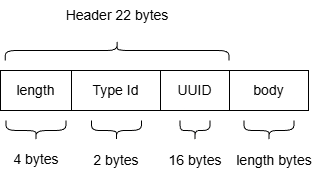
\includegraphics[width=0.9\linewidth]{images/MessageFrame.png}
    \caption{Message Frame used by Transceiver library}
    \label{fig:ambiente-virtual}
\end{figure}

\FloatBarrier

\subsection{Message Serialization}

Serialization is the process that transforms a message into a representation of that message. 
While deserialisation is the process that transforms the representation of the message into the message. 
To ensure that message serialization behaves correctly, it must follow some simple rules:

\begin{itemize}
     \item Both the serializer and deserializer must agree on the exchanged format.
     \item The serialization must be deterministic, always producing the same representation for the same message.
     \item The serialization must be bijective, allowing to rebuild the message from the representation. 
\end{itemize}

As noted before, one advantage of choosing length-prefixed framing is that the body of the message will never contain characters that need to be handled in special cases. 
This is particularly useful since it allows for any arbitrary payload to be exchanged. 
The choice of this type of framing increases the flexibility in the choice of the format of the body. 

The choice of a serialization format is relevant since each message needs to be serialized and deserialized, contributing to a sizable overhead in the message exchange process. 
Formats that minimize the number of bytes needed to represent the object and minimize serialization and deserialization times should therefore be preferred.
Otherwise, other characteristics can be taken into account when choosing a serialization format, 
such as verbosity, readability as in human-readable (text) or machine-readable (binary), adoption, and ease of integration and implementation. 
Given the importance of serialization in message exchange it should be considered as an extensibility point of the library.

\subsection{Protocol Independence}



\setlength\bibitemsep{\baselineskip}
\printbibliography

\end{document}
